\chapter{Results and Discussion}

\section{Performance analysis}

\subsection{Key metrics}

There are three key metrics that will be used to assess system performance impacts: the HTTP response time, throughput, and error rate. Within the context of self-adaptive systems, as described by \citeauthor{weyns_engineering_2018} \cite{weyns_engineering_2018}, there are two levels of a system that can be optimised. Improvements can be made to the inner managed system, or to the outer managing system. For the Ahuora Digital Platform, the optimisation explored here will focus on optimisation of the managing system, or the Kubernetes cluster. These metrics will serve to inform steps towards such optimisation.

\subsubsection{Response time}

The response time for an individual request is the total length of time taken to receive a response from a destination endpoint. This includes the duration of all steps involved in the request, including the time taken to establish an initial connection, perform a TLS handshake, wait for the response, and receive the data. As a metric, it allows an analyst to observe how a system responds over time to increasing load, with a worsening response time indicating that the system is being throttled or is reaching a performance ceiling. From a developer perspective, the response time is important to track, as an increasing response time worsens the experience for users of a product, who may perceive a slowly responding application as a reflection of poor software quality.

\subsubsection{Throughput}

The throughput of a system is the number of requests that are processed per second. This metric can be used to identify the peak capacity of the system, as well as identify the thresholds or points at which system performance degrades. As opposed to the response time, which is concerned with the performance of individual requests, throughput is a metric that provides insight only with respect to behaviour of the overall system. One goal within a performance optimisation context is to maximise the peak throughput of a system to serve more users concurrently.

\subsubsection{Error rate}

Along with speed-oriented metrics like the response time and throughput, it is critical to keep track of the error rate, or the proportion of HTTP requests that failed. Error rates can increase under overloaded system conditions, and can provide early indication that a sustainable throughput threshold has been passed. Another reason to record errors is to ensure that they do not cause invalid observations to be made about test data. In some situations, failed requests may have lower response times than their successful counterparts, which may mislead one to think the system is more responsive than it actually is.

\subsection{Secondary metrics}

\subsubsection{Container-level resource utilisation}

Both CPU and memory usage will provide additional insight into system performance influences. For example, the observation of high consumption of allocated CPU time within a pod or container at the same time as observed request rate instability would possibly indicate the pod is reaching computation limits.

\subsubsection{Cluster-level resource allocation and utilisation}

Especially when auto-scaling policies are in place, it is necessary to track the number of deployed pods for each active cluster deployment. This metric can then be used to calculate the sum of all provisioned resources on the cluster, such as the total requested CPU. With this information, the level of over or under-provisioning can be compared across different workloads, and across workload configuration variations. If a pod requests 2000 millicores of CPU, but only uses 100 millicores on average, then this is a clear sign of severe over-provisioning. Likewise, requesting 500 millicores but quickly reaching an average of 90\% CPU utilisation would indicate under-provisioning. With auto-scaling policies in place, poorly set CPU or memory requests can rapidly multiply into cluster-wide resource allocation issues, such as additional pods being unschedulable.

\subsection{Summary statistics}

Using the data generated within tests, a number of summary statistics for each test result can be derived to assist with immediate comparison of deployment configurations.

\begin{itemize}[itemsep=0pt]
    \item \textbf{Average (mean) request completion rate}: The mean number of requests that were successfully completed per second.
    \item \textbf{Maximum request completion rate}: The peak request completion rate across the test duration.
    \item \textbf{Maximum request start rate}: The peak number of requests started by the k6 test client per second.
    \item \textbf{Average (median) response time}: The median time taken for a request to receive a response.
    \item \textbf{Overall error rate}: The proportion of requests across the test that failed due to an HTTP error or client timeout.
    \item \textbf{Performance degradation threshold}: The point at which the response time exceeds a certain level (100 milliseconds for UOR tests, and 1000 milliseconds for FS tests). This statistic allows for an approximation of the request start and completion rates where system performance begins to degrade rapidly. This threshold will not be calculated for average load or stress load tests.
    \item \textbf{Maximum started and completed request ratio}: The largest ratio between the number of requests that have started and the number that have completed. A high ratio indicates that the system is failing to process as many requests as it is receiving. This will not be calculated for breakpoint load tests.
    \item \textbf{Maximum cluster CPU request proportion}: The peak proportion of available cluster CPU used by a deployment. This will be calculated for the Django and IDAES pods only, and only for the resource allocation and utilisation tests.
\end{itemize}

\subsection{Rolling window statistics}

Response times will be assessed using an exponentially-weighted moving average (EWMA), along with comparisons at different moving percentiles. Use of a rolling median would appear either too unstable with a small window, or lag behind in showing recent trends. Using an EWMA allows recent data to be paid more attention, and enables better correlation analysis to be conducted.

\section{Unit operation retrieval (UOR) experiment results}

\subsection{Benchmarks}

\begin{figure}[H]
    
    \centering
    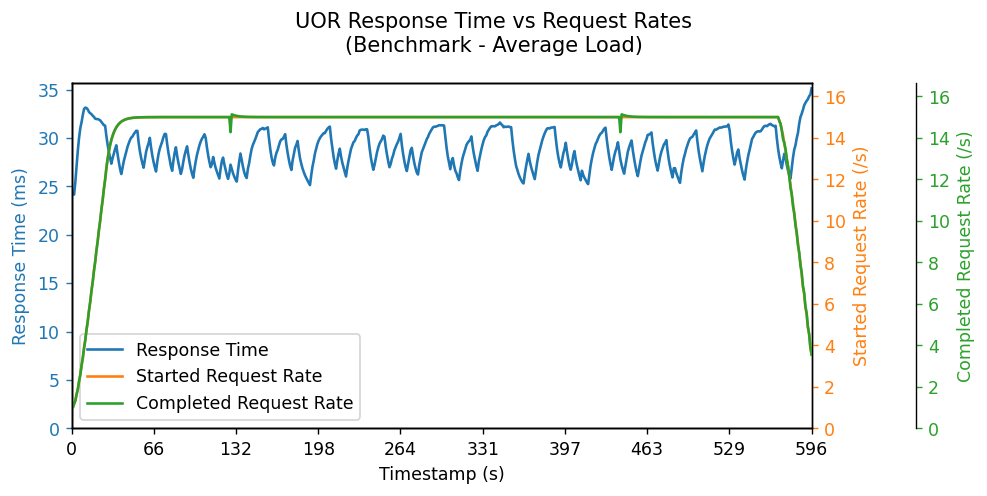
\includegraphics[width=0.8\textwidth]{figures/uor-benchmark-average.png}
    \caption{UOR response time vs. request rate graph - average load benchmark}
    \label{figure:uor-benchmark-average}
\end{figure}

Both response time and request rate degradation can be observed in the local spike test (Fig. \ref{figure:uor-benchmark-spike}). After reaching \textasciitilde40 requests per second, the response time rapidly increases, and the request completion rate starts to diverge from the request start rate. At 45 requests per second (RPS), the response time average increases past 100 milliseconds, and reaches tens of thousands of milliseconds as the request rate continues to increase. During the test, the request start rate is also seen degrading (between 135 and 189 seconds). This is because of the virtual user limit of 2000 set on the k6 test client, which was configured to prevent system resource starvation by the test client. The response time does not appear to recover towards the end of the test. Approximately 0.036\% of requests in the spike tests failed, while neither the average or stress load tests had any failed requests.

\begin{figure}[H]
    \centering
    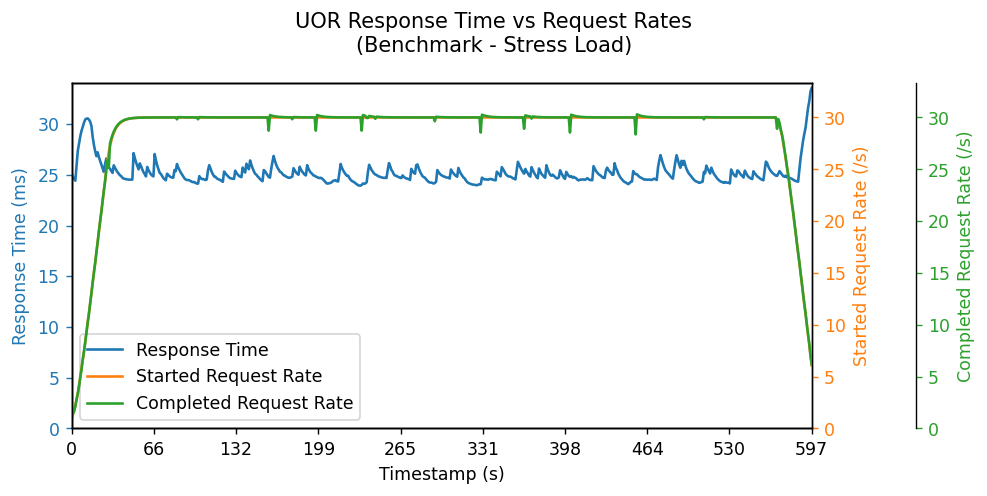
\includegraphics[width=0.8\textwidth]{figures/uor-benchmark-stress.png}
    \caption{UOR response time vs. request rate graph - stress load benchmark}
    \label{figure:uor-benchmark-stress}
\end{figure}

\begin{figure}[H]
    \centering
    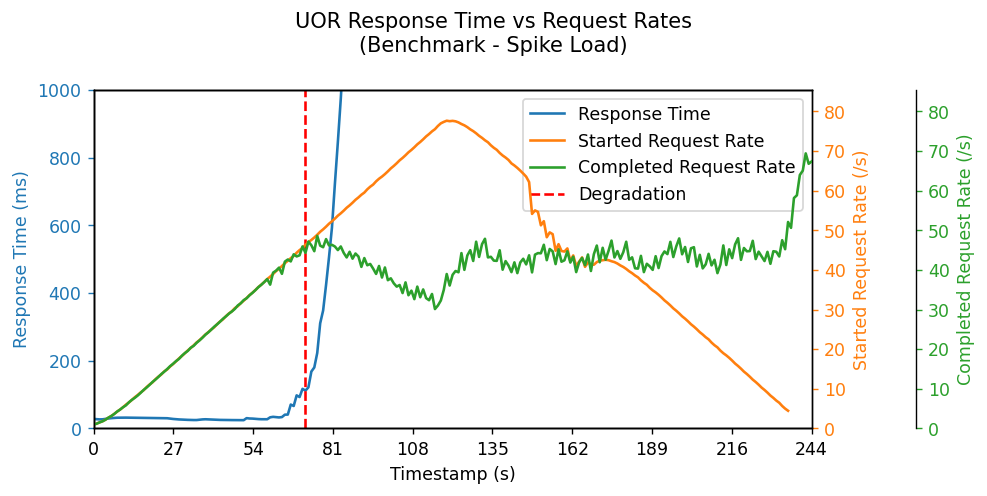
\includegraphics[width=0.8\textwidth]{figures/uor-benchmark-spike.png}
    \caption{UOR response time vs. request rate graph - spike load benchmark}
    \label{figure:uor-benchmark-spike}
\end{figure}

The breakpoint test (Fig. \ref{figure:uor-benchmark-breakpoint}) also identifies this same 45 RPS threshold, beyond which the average response time exceeds 100 milliseconds, and the request completion rate also diverges. No requests failed in the breakpoint tests, but this in part due to the early termination threshold used by breakpoint tests.

\begin{figure}[H]
    \centering
    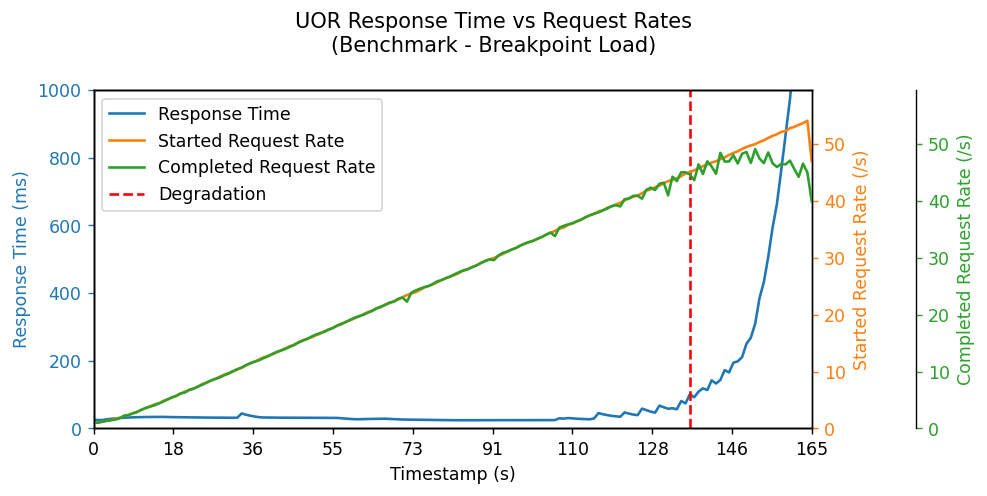
\includegraphics[width=0.8\textwidth]{figures/uor-benchmark-breakpoint.png}
    \caption{UOR response time vs. request rate graph - breakpoint load benchmark}
    \label{figure:uor-benchmark-breakpoint}
\end{figure}



\subsection{Replica count}

\begin{figure}[h]
    \centering
    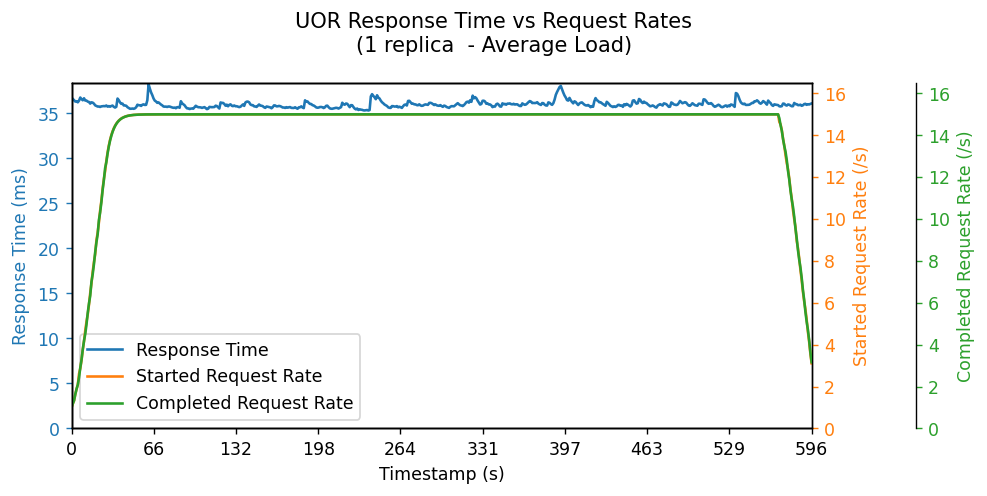
\includegraphics[width=0.8\textwidth]{figures/uor-replica-count-i1-average.png}
    \caption{UOR response time vs. request rate graph - breakpoint load with one replica}
    \label{figure:uor-replica-count-i1-average}
\end{figure}

Using an average load profile against a Django deployment configuration with one replica allows some differences to be observed between the average load benchmark and this cluster-bound test. While the response time of the benchmark sits between 25 and 30 milliseconds, the single replica test sees a median average response time of 35.74 milliseconds (Fig. \ref{figure:uor-replica-count-i1-average}).

\begin{figure}[h]
    \centering
    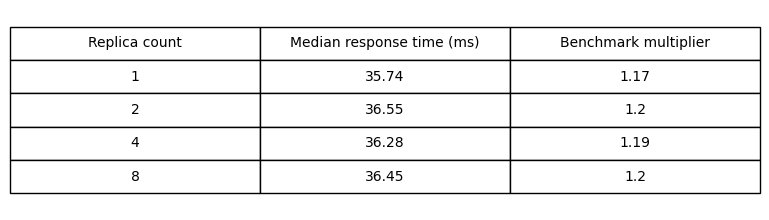
\includegraphics[width=0.8\textwidth]{figures/uor-replica-count-rt-comparison.png}
    \caption{Table of median response times by replica count, average load}
    \label{figure:uor-replica-count-rt-comparison}
\end{figure}

This higher response time average is consistent with any number of replicas (as seen in Fig. \ref{figure:uor-replica-count-rt-comparison}) when average load is applied. The simple explanation for this difference is the use of TLS in the HTTPS connections used between the test client and the cluster, which may take between 5 and 10 milliseconds per request. Unencrypted HTTP is used to access the local deployment, so less work is required to establish a connection. As well as this, the 5 millisecond artificial delay added for cluster-bound requests partially accounts for this discrepancy. A similar range of averages is observed within the replica count stress tests, albeit with a larger gap between the benchmark and replica count median response times (due to the lower average achieved by the benchmark in stress tests compared with the average load tests.)

\begin{figure}[h]
    \centering
    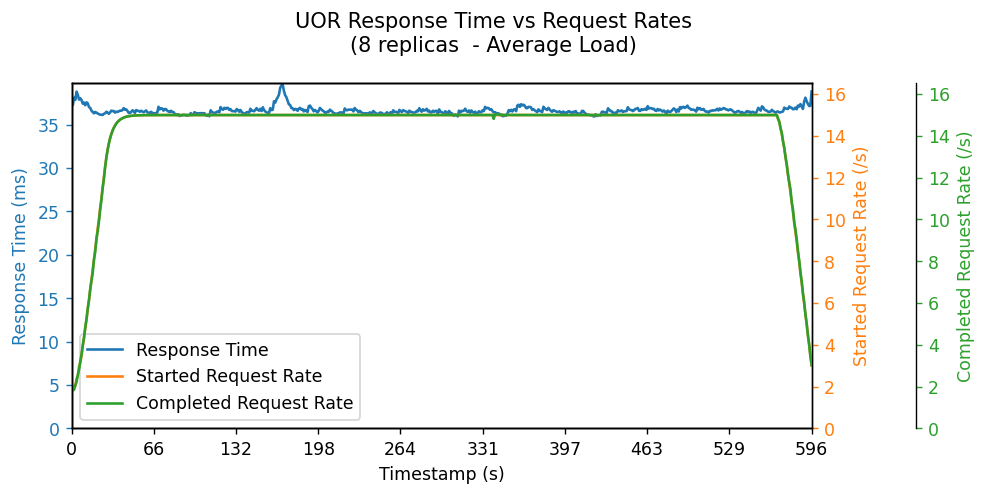
\includegraphics[width=0.8\textwidth]{figures/uor-replica-count-i4-average.png}
    \caption{UOR response time vs. request rate graph - breakpoint load with eight replicas}
    \label{figure:uor-replica-count-i4-average}
\end{figure}

Regardless, any tested number of Django replicas running on the cluster is able to process incoming requests as fast as they arrive (evidenced in Fig \ref{figure:uor-replica-count-i1-average} and \ref{figure:uor-replica-count-i4-average}), so there are no significant request rate differences between the benchmarks and the replica count experiments. However, where the benchmarked local deployment shows evidence of performing worse than the clustered deployment is when testing spike and breakpoint loads with more than one replica. As shown in Fig. \ref{figure:uor-replica-count-rt-comp-spike}, a replica count of one performs similar to the benchmark, where the median response time reaches almost 17,000 milliseconds. The median response times for the remaining replica counts (2, 4 and 8) are magnitudes lower, ranging from 39.89 to 42.14 milliseconds.

\begin{figure}[h]
    \centering
    \begin{subfigure}{.5\textwidth}
      \centering
      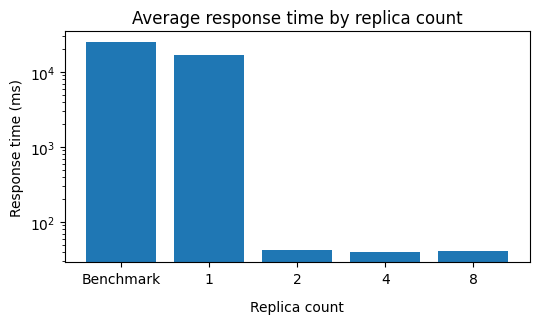
\includegraphics[width=\linewidth]{figures/uor-replica-count-rt-comp-spike1.png}
      \caption{Logarithmic scale}
    \end{subfigure}%
    \begin{subfigure}{.5\textwidth}
      \centering
      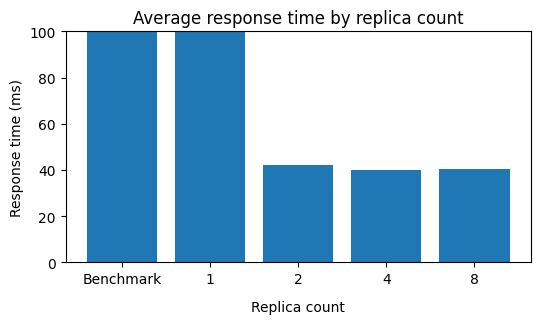
\includegraphics[width=\linewidth]{figures/uor-replica-count-rt-comp-spike2.png}
      \caption{Linear scale}
    \end{subfigure}

    \caption{Median response times by replica count (spike load)}
    \label{figure:uor-replica-count-rt-comp-spike}
\end{figure}

With either four or eight Django replicas, the average response time increases by almost 30\% at the peak request arrival rate (Fig. \ref{figure:uor-replica-count-graph}), but the system is otherwise able to process these requests at the arrival rate. Early signs of degradation are seen when using two replicas, with the response time sharply doubling at the peak request rate, though both request rate curves are mostly consistent \ref{figure:uor-replica-count-graph2}. Interestingly, the response time curve dampening effect with four replicas is highly similar to that with eight replicas, despite doubling the number of available workers. With one replica, this is not the case, having a similar request completion curve (Fig. \ref{figure:uor-replica-count-graph2}) to the benchmark (Fig. \ref{figure:uor-benchmark-spike}), along with an 8.79\% request fail rate, which is 246.35 times worse than the benchmark. The usage of one replica results in the same degradation request rate as the benchmark. None of the other replica count variants have a degradation request rate. When it comes to the started and completed request ratio, a single replica sees a maximum ratio of 1.34 started requests to completed requests, whereas the other replica counts all reach no more than 1.02.

\begin{figure}[H]
    \centering
    \begin{subfigure}{.5\textwidth}
      \centering
      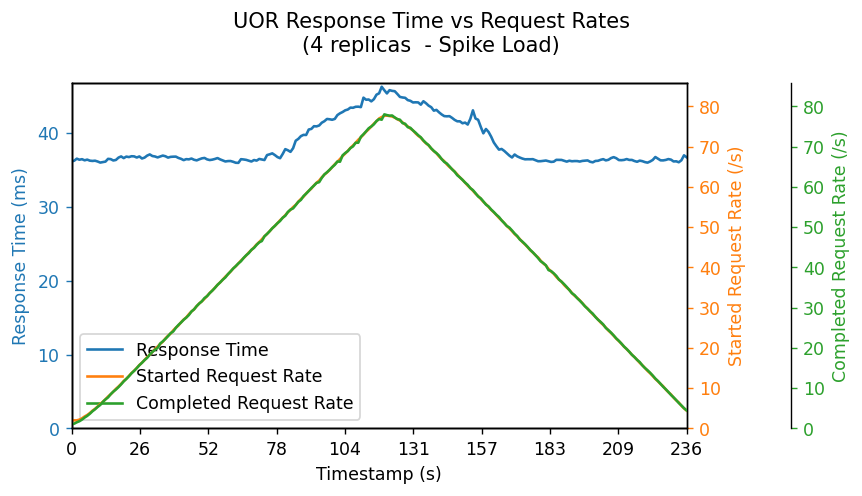
\includegraphics[width=\linewidth]{figures/uor-replica-count-i3-graph.png}
      \caption{4 replicas}
    \end{subfigure}%
    \begin{subfigure}{.5\textwidth}
      \centering
      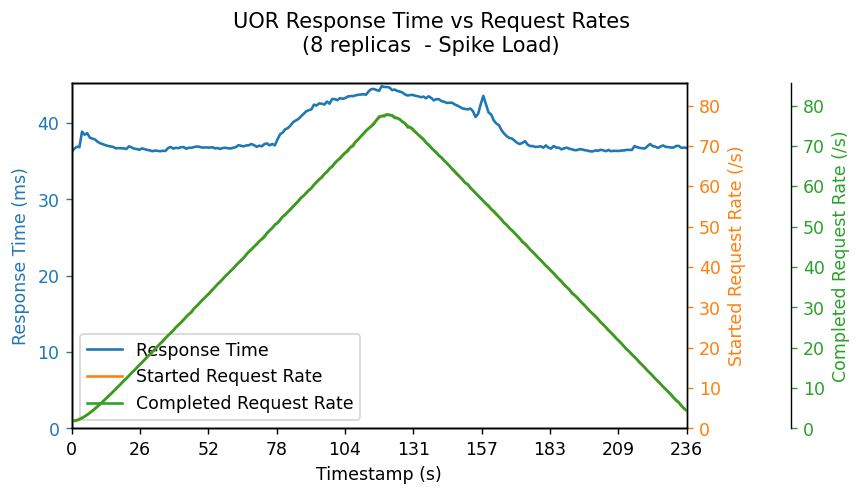
\includegraphics[width=\linewidth]{figures/uor-replica-count-i4-graph.png}
      \caption{8 replicas}
    \end{subfigure}

    \caption{Response time vs. request rate graph (spike load, 4 and 8 replicas)}
    \label{figure:uor-replica-count-graph}
\end{figure}

\begin{figure}[h]
    \centering
    \begin{subfigure}{.5\textwidth}
      \centering
      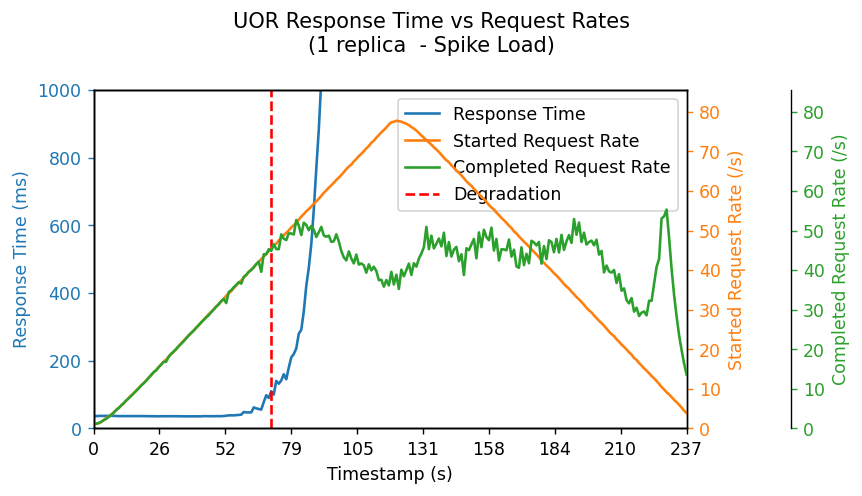
\includegraphics[width=\linewidth]{figures/uor-replica-count-i1-graph.png}
      \caption{1 replica}
    \end{subfigure}%
    \begin{subfigure}{.5\textwidth}
      \centering
      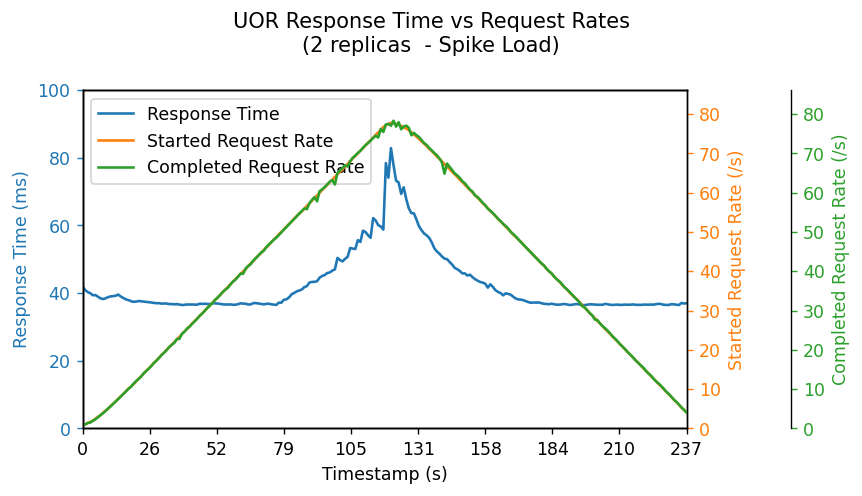
\includegraphics[width=\linewidth]{figures/uor-replica-count-i2-graph.png}
      \caption{2 replicas}
    \end{subfigure}

    \caption{Response time vs. request rate graph (spike load, 1 and 2 replicas)}
    \label{figure:uor-replica-count-graph2}
\end{figure}

Within the breakpoint tests, there is a significant distinction between the maximum request start rate reached across the lowest and highest number of replicas. As visible in Fig. \ref{figure:uor-replica-count-graph-breakpoint}, an eight-replica Django deployment reaches \textasciitilde150 started RPS (3.36 times the benchmark) before the response time exceeds 1000 milliseconds. On the other hand, the single replica deployment passes the degradation threshold at \textasciitilde35.3 started RPS. Over the course of the eight replica breakpoint test, the response time gradually increases with the request rate, becoming more unstable over time. Fig. \ref{figure:uor-replica-count-breakpoint-max-reqs} shows that a start RPS of 158 (2.84 times the benchmark) is the maximum reached by the eight-replica deployment. The four-replica deployment reaches a slightly smaller limit of 157 RPS, though it has a lower degradation request rate of \textasciitilde136.4 RPS (Fig. \ref{figure:uor-replica-count-breakpoint-deg-rates}).

\begin{figure}[h]
    \centering
    \begin{subfigure}{.5\textwidth}
      \centering
      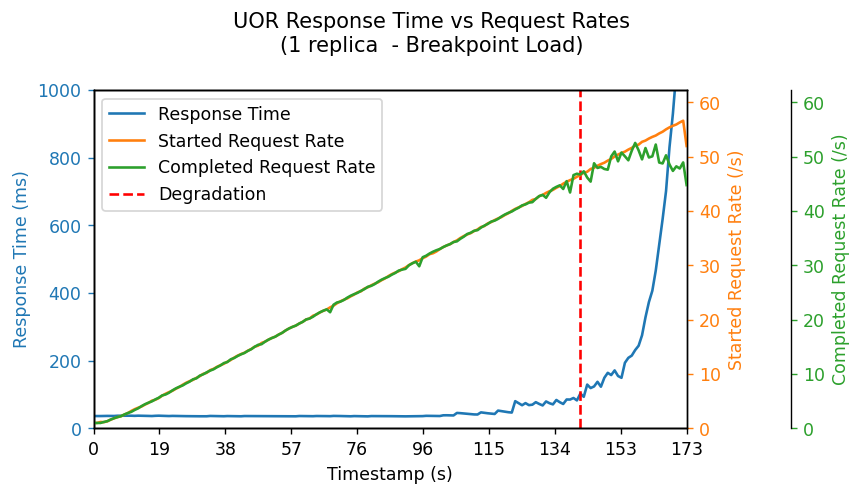
\includegraphics[width=\linewidth]{figures/uor-replica-count-i1-graph-breakpoint.png}
      \caption{1 replica}
    \end{subfigure}%
    \begin{subfigure}{.5\textwidth}
      \centering
      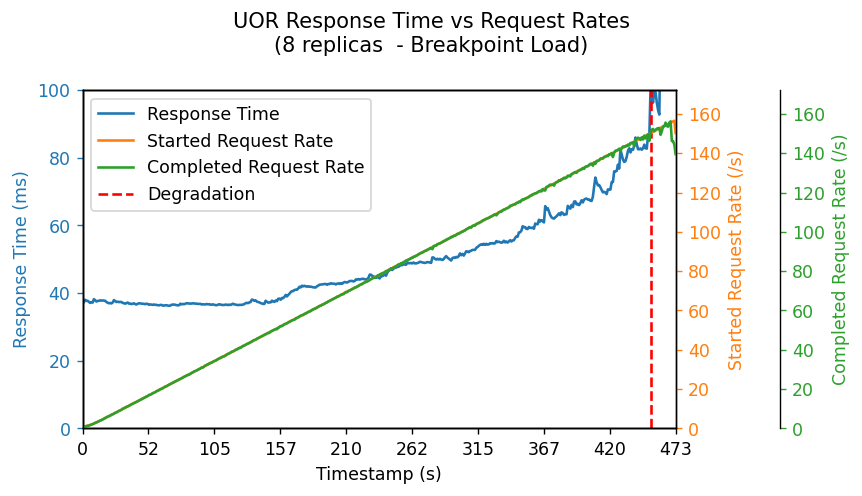
\includegraphics[width=\linewidth]{figures/uor-replica-count-i4-graph-breakpoint.png}
      \caption{8 replicas}
    \end{subfigure}

    \caption{Response time vs. request rate graph (breakpoint load, 1 and 8 replicas)}
    \label{figure:uor-replica-count-graph-breakpoint}
\end{figure}

\begin{figure}[h]
    \centering
    \begin{minipage}{.45\textwidth}
      \centering
      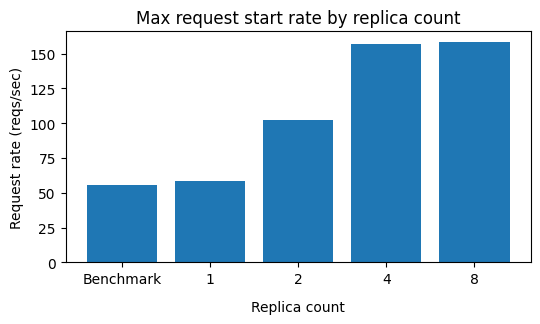
\includegraphics[width=\linewidth]{figures/uor-replica-count-breakpoint-max-reqs.png}

      \caption{Chart of maximum request start rates by replica count}
      \label{figure:uor-replica-count-breakpoint-max-reqs}
    \end{minipage}%
    \hspace{0.09\textwidth} % Adjust the horizontal space here
    \begin{minipage}{.45\textwidth}
      \centering
      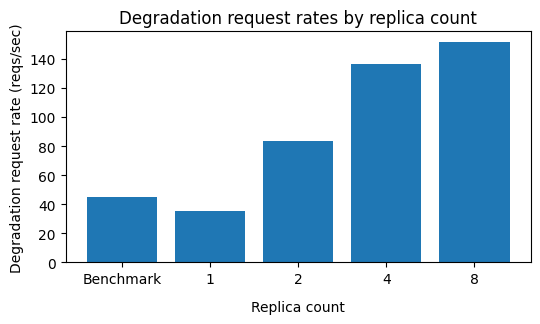
\includegraphics[width=\linewidth]{figures/uor-replica-count-breakpoint-deg-rates.png}

      \caption{Chart of degradation request rates by replica count}
      \label{figure:uor-replica-count-breakpoint-deg-rates}
    \end{minipage}
\end{figure}

In general, a higher number of replicas allows for a higher degradation threshold, though when it comes to the maximum start RPS, the relationship does not appear to be as straightforward. The maximum start RPS only slightly increases from four to eight replicas, which indicates there may be a bottleneck elsewhere in the system preventing a higher maximum.

\subsection{Resource allocation and utilisation}

Results based on a static number of replicas have been showcased, but the effect of dynamic replica auto-scaling on key system metrics is also assessed.

% \subsection{Minimum replicas}
% \subsubsection{Average load}
% \subsubsection{Stress load}
% \subsubsection{Spike load}
% \subsubsection{Breakpoint load}

\section{Flowsheet solving (FS) experiment results}

\subsection{Benchmarks}


\subsection{Replica count}


\subsection{Resource allocation and utilisation}


% \subsection{Minimum replicas}
% \subsubsection{Average load}
% \subsubsection{Stress load}
% \subsubsection{Spike load}
% \subsubsection{Breakpoint load}

\section{Impacts}
Efficiency, accuracy, feasibility (examples of demonstrable impacts).
\section{Threats to validity}